\documentclass{beamer}
\usetheme{Boadilla}

\makeatother
\setbeamertemplate{footline}
{
    \leavevmode%
    \hbox{%
    \begin{beamercolorbox}[wd=.4\paperwidth,ht=2.25ex,dp=1ex,center]{author in head/foot}%
        \usebeamerfont{author in head/foot}\insertshortauthor
    \end{beamercolorbox}%
    \begin{beamercolorbox}[wd=.55\paperwidth,ht=2.25ex,dp=1ex,center]{title in head/foot}%
        \usebeamerfont{title in head/foot}\insertshorttitle
    \end{beamercolorbox}%
    \begin{beamercolorbox}[wd=.05\paperwidth,ht=2.25ex,dp=1ex,center]{date in head/foot}%
        \insertframenumber{}
    \end{beamercolorbox}}%
    \vskip0pt%
}
\makeatletter
\setbeamertemplate{navigation symbols}{}

\usepackage[T1]{fontenc}
\usepackage{lmodern}
\usepackage{amssymb,amsmath}
\renewcommand{\familydefault}{\sfdefault}

\usepackage{mathtools}
\usepackage{graphicx}
\usepackage{threeparttable}
\usepackage{booktabs}
\usepackage{siunitx}
\sisetup{parse-numbers=false}

%\setlength{\OuterFrameSep}{-2pt}
%\makeatletter
%\preto{\@verbatim}{\topsep=-10pt \partopsep=-10pt }
%\makeatother

\title[Lecture 4:\ Logit Model I]{Lecture 4:\ Logit Model I}
\author[ResEcon 703:\ Advanced Econometrics]{ResEcon 703:\ Topics in Advanced Econometrics}
\date{Matt Woerman\\University of Massachusetts Amherst}

\begin{document}

{\setbeamertemplate{footline}{} 
\begin{frame}[noframenumbering]
    \titlepage
\end{frame}
}

\begin{frame}\frametitle{Agenda}
    Last time
    \begin{itemize}
        \item Random Utility Model
    \end{itemize}
    \vspace{2ex}
    Today
    \begin{itemize}
    	\item Logit Model
    	\item Binary Logit Model
    	\item Some Logit Properties
    	\item Binary Logit Model Example in R
    	\item Gruber and Poterba (1994)
    \end{itemize}
    \vspace{2ex}
    Upcoming
    \begin{itemize}
        \item Reading for next time
        \begin{itemize}
            \item Adamowicz et al. (1994)
        \end{itemize}
        \item Problem set
        \begin{itemize}
            \item Problem Set 1 is posted, due September 24
        \end{itemize}
    \end{itemize}
\end{frame}

\begin{frame}\frametitle{Random Utility Model Recap}
    A decision maker chooses the alternative that maximizes utility
    \begin{itemize}
		\item A decision maker, $n$, faces a choice among $J$ alternatives
    	\item Alternative $j$ provides utility $U_{nj}$ (where $j = 1, \ldots, J$)
    	\item $n$ chooses $i$ if and only if $U_{ni} > U_{nj} \; \forall j \neq i$
   	\end{itemize}
   	\vspace{2ex}
   	We model utility as having observed and unobserved components
   	\begin{itemize}
		\item Observed factors: $V_{nj}$
		\item Unobserved factors: $\varepsilon_{nj}$
	\end{itemize}
	$$U_{nj} = V_{nj} + \varepsilon_{nj}$$ \\
	\vspace{2ex}
	The probability the decision maker chooses alternative $i$ is
    \begin{align*}
    	P_{ni} &= \Pr(U_{ni} > U_{nj} \; \forall j \neq i) \\
    	&= \int_\varepsilon I(\varepsilon_{nj} - \varepsilon_{ni} < V_{ni} - V_{nj} \; \forall j \neq i) f(\varepsilon_n) d\varepsilon_n
    \end{align*}
\end{frame}

\begin{frame}\frametitle{}
    \vfill
    \centering
    \begin{beamercolorbox}[center]{title}
        \Large Logit Model
    \end{beamercolorbox}
    \vfill
\end{frame}

\begin{frame}\frametitle{Logit Model}
    The logit model makes a (somtimes overly) simple assumption about the joint density of unobserved utility, $f(\varepsilon_n)$
    $$\varepsilon_{nj} \sim \text{i.i.d.\ type I extreme value (Gumbel) with } Var(\varepsilon_{nj}) = \frac{\pi^2}{6}$$ \\
    \vspace{3ex}
    Why make this assumption about the unobserved utility of alternatives?
    \begin{itemize}
    	\item It yields choice probabilities that have a closed-form expression
    \end{itemize}
\end{frame}

\begin{frame}\frametitle{Type I Extreme Value Density and Distribution}
    Type I extreme value is similar to a normal distribution but with a fatter tail on one side \\
    \begin{columns}
		\begin{column}{0.5\textwidth}
			\begin{center}
				Probability density
				$$f(\varepsilon_{nj}) = e^{-\varepsilon_{nj}} e^{-e^{-\varepsilon_{nj}}}$$
				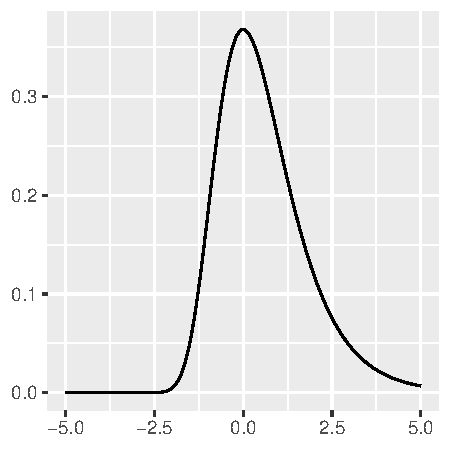
\includegraphics[width=0.8\textwidth]{ev_pdf.pdf}      
			\end{center}
		\end{column}
		\begin{column}{0.5\textwidth}
    		\begin{center}
     			Cumulative distribution 
     			$$F(\varepsilon_{nj}) = e^{-e^{-\varepsilon_{nj}}}$$
				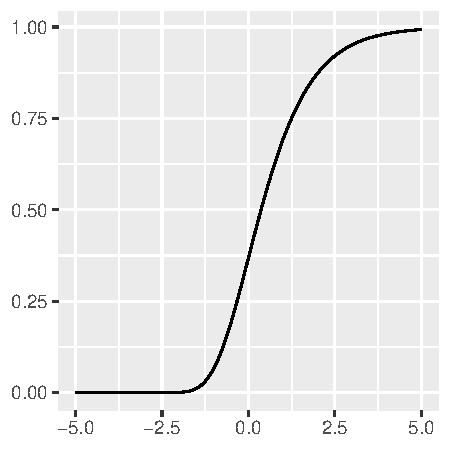
\includegraphics[width=0.8\textwidth]{ev_cdf.pdf}          
     		\end{center}
		\end{column}
	\end{columns}
\end{frame}

\begin{frame}\frametitle{Logistic Density and Distribution}
    The difference of two type I extreme value draws, $\varepsilon_{nji}^* = \varepsilon_{nj} - \varepsilon_{ni}$, follows the logistic distribution
    \begin{columns}
		\begin{column}{0.5\textwidth}
			\begin{center}
				Probability density \\
				\vspace{-4ex}
				$$f(\varepsilon_{nji}^*) = \frac{e^{\varepsilon_{nji}^*}}{\left( 1 + e^{\varepsilon_{nji}^*} \right)^2}$$ \\
				\vspace{-2ex}
				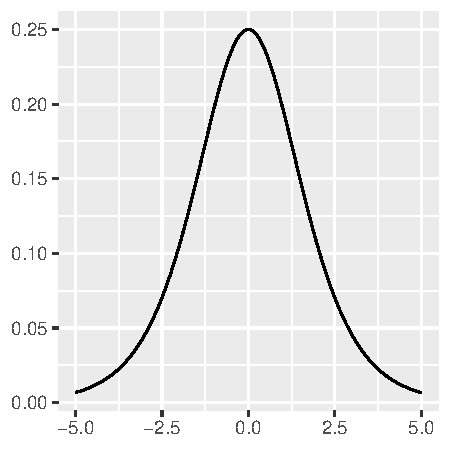
\includegraphics[width=0.8\textwidth]{logistic_pdf.pdf}      
			\end{center}
		\end{column}
		\begin{column}{0.5\textwidth}
    		\begin{center}
     			Cumulative distribution \\
     			\vspace{-4ex}
     			$$F(\varepsilon_{nji}^*) = \frac{e^{\varepsilon_{nji}^*}}{1 + e^{\varepsilon_{nji}^*}}$$ \\
     			\vspace{0ex}
				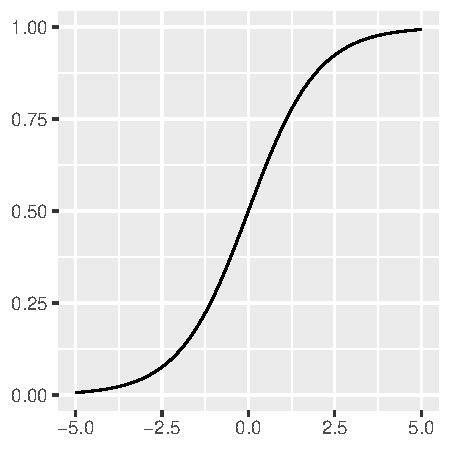
\includegraphics[width=0.8\textwidth]{logistic_cdf.pdf}          
     		\end{center}
		\end{column}
	\end{columns}
\end{frame}

\begin{frame}\frametitle{Logit Choice Probabilities}
	\vspace{-4ex}
    \begin{align*}
    	P_{ni} &= \Pr(U_{ni} > U_{nj} \; \forall j \neq i) \\
    	&= \Pr(V_{ni} + \varepsilon_{ni} > V_{nj} + \varepsilon_{nj} \; \forall j \neq i) \\
    	&= \Pr(\varepsilon_{nj} < \varepsilon_{ni} + V_{ni} - V_{nj} \; \forall j \neq i) \\
    	\intertext{For a given $\varepsilon_{ni}$, this is the cumulative distribuion of each $\varepsilon_{nj}$, and because $\varepsilon_{nj}$ is i.i.d.}	 
    	P_{ni} \mid \varepsilon_{ni} &= \prod_{j \neq i} e^{-e^{-(\varepsilon_{ni} + V_{ni} - V_{nj})}} \\
    	\intertext{But $\varepsilon_{ni}$ is random, so we have to integrate over the density of $\varepsilon_{ni}$}
    	P_{ni} &= \int \left( \prod_{j \neq i} e^{-e^{-(\varepsilon_{ni} + V_{ni} - V_{nj})}} \right) e^{-\varepsilon_{ni}} e^{-e^{-\varepsilon_{ni}}} d\varepsilon_{ni} \\
    	&= \frac{e^{V_{ni}}}{\sum_j e^{V_{nj}}}
    \end{align*}
    The probability of $n$ choosing $i$ is a closed-form expression that depends on the representative utility (or observable components) of all alternatives
\end{frame}

\begin{frame}\frametitle{Representative Utility}
    We usually specify representative utility as a linear function of observable characteristics of the alternative and the agent
    $$V_{nj} = \beta' x_{nj}$$ \\
    \begin{itemize}
    	\item A linear function is highly flexible and can include interactions, squared terms, etc.
    	\item Most utility functions can be closely approximated by a function that is linear in parameters
    	\item Non-linear utility can greatly complicate estimation
    \end{itemize}
    \vspace{3ex}
    With linear representative utility, the logit choice probability is
    $$P_{ni} = \frac{e^{\beta' x_{ni}}}{\sum_j e^{\beta' x_{nj}}}$$
\end{frame}

\begin{frame}\frametitle{Properties of Logit Choice Probabilities}
    $P_{ni}$ is always within the range $(0, 1)$
    \begin{itemize}
    	\item $P_{ni} \rightarrow 1$ as $V_{ni} \rightarrow \infty$
    	\item $P_{ni} \rightarrow 0$ as $V_{ni} \rightarrow -\infty$
    \end{itemize}
    \vspace{2ex}
    Choice probabilities sum to 1
    $$\sum_{i = 1}^J P_{ni} = \sum_{i = 1}^J \frac{e^{V_{ni}}}{\sum_j e^{V_{nj}}} =\frac{\sum_i e^{V_{ni}}}{\sum_j e^{V_{nj}}} = 1$$ \\
    \vspace{2ex}
    Choice probability is a sigmoidal function of representative utility (see the logistic CDF)
    \begin{itemize}
    	\item Marginal effects are small when probabilities are close to 0 or 1
    	\item Marginal effects are largest when $P_{ni} = 0.5$
    \end{itemize}
\end{frame}

\begin{frame}\frametitle{}
    \vfill
    \centering
    \begin{beamercolorbox}[center]{title}
        \Large Binary Logit Model
    \end{beamercolorbox}
    \vfill
\end{frame}

\begin{frame}\frametitle{Binary Logit Model}
    With only two choices, the logit choice probabilities simplify to
    \begin{align*}
    	P_{n1} &= \frac{e^{V_{n1}}}{e^{V_{n1}} + e^{V_{n2}}} \\
    	P_{n2} &= \frac{e^{V_{n2}}}{e^{V_{n1}} + e^{V_{n2}}}
    \end{align*}
    The log odds ratio of alternative 1 is
    $$\ln \left( \frac{P_{n1}}{1 - P_{n1}} \right) = V_{n1} - V_{n2}$$
    If we assume representative utility is linear, $V_{ni} = \beta' x_{ni}$
    $$\ln \left( \frac{P_{n1}}{1 - P_{n1}} \right) = \beta' (x_{n1} - x_{n2})$$
    The log odds ratio of each alternative is a linear function of $\beta$ and $x_n$
    \begin{itemize}
    	\item \texttt{glm()} with \texttt{family = "binomial"} can estimate this model
    \end{itemize}
\end{frame}

\begin{frame}\frametitle{Binary Logit Choice Probabilities Example}
    A person chooses whether to take a car ($c$) or a bus ($b$) to work
    \begin{itemize}
    	\item We observe the time, $T$, and cost, $M$, of each choice
    \end{itemize}
    \vspace{1ex}
    We specify the representative utility of each alternative as
    \begin{align*}
    	V_c &= \alpha T_c + \beta M_c \\
    	V_b &= \alpha T_b + \beta M_b
    \end{align*}
    Using the logit model, the probability of driving is
    $$P_c = \frac{e^{\alpha T_c + \beta M_c}}{e^{\alpha T_c + \beta M_c} + e^{\alpha T_b + \beta M_b}}$$
    and the log odds ratio of driving is
    $$\ln \left( \frac{P_c}{1 - P_c} \right) = (\alpha T_c + \beta M_c) - (\alpha T_b + \beta M_b)$$
\end{frame}

\begin{frame}\frametitle{}
    \vfill
    \centering
    \begin{beamercolorbox}[center]{title}
        \Large Some Logit Properties
    \end{beamercolorbox}
    \vfill
\end{frame}

\begin{frame}\frametitle{Marginal Effects}
    Unlike a linear probability model, the coefficients of a logit model cannot be interpreted as marginal effects on probability
    \begin{itemize}
    	\item Instead, they give the marginal utility of the corresponding variable
    	\item We know the choice probabilities, so we can derive marginal effects!
    \end{itemize}
    \vspace{2ex}
    The marginal effect of $z_{ni}$, an observed factor of alternative $i$, on $P_{ni}$, the probability that agent $n$ chooses alternative $i$
    \begin{align*}
    	\frac{\partial P_{ni}}{\partial z_{ni}} &= \frac{\partial \left( e^{V_{ni}} / \sum_j e^{V_{nj}} \right)}{\partial z_{ni}} \\
    	&= \frac{\partial V_{ni}}{\partial z_{ni}} P_{ni} (1 - P_{ni}) \\
    	\intertext{If $V_{ni}$ is linear in $z_{ni}$ with coefficient $\beta_z$, then the marginal effect is}
    	\frac{\partial P_{ni}}{\partial z_{ni}} &= \beta_z P_{ni} (1 - P_{ni})
    \end{align*}
\end{frame}

\begin{frame}\frametitle{Cross Marginal Effects}
    The marginal effect of $z_{nj}$, an observed factor of alternative $j$, on $P_{ni}$, the probability that agent $n$ chooses alternative $i$
    \begin{align*}
    	\frac{\partial P_{ni}}{\partial z_{nj}} &= \frac{\partial \left( e^{V_{ni}} / \sum_k e^{V_{nk}} \right)}{\partial z_{nj}} \\
    	&= -\frac{\partial V_{nj}}{\partial z_{nj}} P_{ni} P_{nj} \\
    	\intertext{If $V_{nj}$ is linear in $z_{nj}$ with coefficient $\beta_z$, then the marginal effect is}
    	\frac{\partial P_{ni}}{\partial z_{nj}} &= -\beta_z P_{ni} P_{nj}
    \end{align*} \\
    \vspace{1ex}
    In a binary logit model, these marginal effect expressions are negatives of each another
\end{frame}

\begin{frame}\frametitle{Elasticities}
    Sometimes elasticities are more informative than marginal effects, especially when considering price changes \\
    \vspace{3ex}
    The elasticity of $P_{ni}$, the probability that agent $n$ chooses alternative $i$, with respect to $z_{ni}$, an observed factor of alternative $i$
    \begin{align*}
    	E_{iz_{ni}} &= \frac{\partial P_{ni}}{\partial z_{ni}} \frac{z_{ni}}{P_{ni}} \\
    	&= \frac{\partial V_{ni}}{\partial z_{ni}} z_{ni} (1 - P_{ni}) \\
    	\intertext{If $V_{nj}$ is linear in $z_{nj}$ with coefficient $\beta_z$, then the elasticity is}
    	E_{iz_{ni}} &= \beta_z z_{ni} (1 - P_{ni})
    \end{align*}
\end{frame}

\begin{frame}\frametitle{Cross Elasticities}
    The elasticity of $P_{ni}$, the probability that agent $n$ chooses alternative $i$, with respect to $z_{nj}$, an observed factor of alternative $j$
    \begin{align*}
    	E_{iz_{nj}} &= \frac{\partial P_{ni}}{\partial z_{nj}} \frac{z_{nj}}{P_{ni}} \\
    	&= -\frac{\partial V_{nj}}{\partial z_{nj}} z_{nj} P_{nj} \\
    	\intertext{If $V_{nj}$ is linear in $z_{nj}$ with coefficient $\beta_z$, then the elasticity is}
    	E_{iz_{nj}} &= -\beta_z z_{nj} P_{nj}
    \end{align*} \\
    \vspace{1ex}
    This elasticity depends only on features of alternative $j$ and not on features of alternative $i$
\end{frame}

\begin{frame}\frametitle{Taste Variation}
    Decision makers' tastes can vary for many reasons, some of which are observable and others are not
    \begin{itemize}
    	\item The logit model can only explicitly capture taste variation due to observable characteristics 
    \end{itemize}
    \vspace{2ex}
    Consider some sources of taste variation in the car vs.\ bus example
    \begin{itemize}
    	\item Some people hate driving and some people love it, but we do not directly observe this preference
    	\begin{itemize}
    		\item We cannot explicitly include this taste variation in the model $\ldots$ yet!
    	\end{itemize}
    	\item People with higher incomes care less about the cost of each alternative
    \end{itemize}
    $$\beta_n = \frac{\beta}{I_n} \quad \Rightarrow \quad U_{nc} = \alpha T_{nc} + \beta \frac{M_{nc}}{I_n} + \varepsilon_{nc}$$
\end{frame}

\begin{frame}\frametitle{Scale Parameter}
    We assume the utility of unobserved factors has variance $\pi^2 / 6$
    \begin{itemize}
    	\item We can use a scale parameter, $\sigma$, to allow for a different variance \\
    \end{itemize}
    \vspace{2ex}
    Suppose the unobserved portion of utility actually has variance $\sigma^2 \times (\pi^2 / 6)$
    $$U_{nj}^* = V_{nj} + \varepsilon_{nj}^*$$
    Dividing by $\sigma$ gives a scaled model
    $$U_{nj} = \frac{V_{nj}}{\sigma} + \varepsilon_{nj} \text{ where } \varepsilon_{nj} = \frac{\varepsilon_{nj}^*}{\sigma}$$
    The variance of this scaled unobserved component is
    $$Var(\varepsilon_{nj}) = \frac{1}{\sigma^2} Var(\varepsilon_{nj}^*) = \frac{\pi^2}{6}$$
\end{frame}

\begin{frame}\frametitle{Logit Choice Probabilities with a Scale Parameter}
    In the scaled model, choice probabilities are
    \begin{align*}
    P_{ni} &= \frac{e^{V_{ni} / \sigma}}{\sum_j e^{V_{nj} / \sigma}} \\
    \intertext{If $V_{nj}$ is linear in parameters with coefficients $\beta^*$}
    P_{ni} &= \frac{e^{(\beta^* / \sigma)' x_{ni}}}{\sum_j e^{(\beta^* / \sigma)' x_{nj}}}
    \intertext{But $\beta^*$ and $\sigma$ are not separately identified, so we can only estimate their ratio, $\beta = \beta^* / \sigma$, which gives the standard logit expression}
    P_{ni} &= \frac{e^{\beta' x_{ni}}}{\sum_j e^{\beta' x_{nj}}}
    \end{align*}
    Parameters are estimated relative to the variance of unobserved utility
\end{frame}

\begin{frame}\frametitle{Heteroskedasticity and the Scale Parameter}
    Different subsets of decision makers may each have a different variance of unobserved utility
    \begin{itemize}
    	\item We can use scale parameters to account for this group-wise heteroskedasticity
    	\item We can estimate the relative scale parameters of each group compared to one reference group
    \end{itemize}
    \vspace{2ex}
    Suppose we have commute data for both Amherst ($A$) and Boston ($B$)
    \begin{itemize}
    	\item The scale parameters for each city are $\sigma^A$ and $\sigma^B$ with $k = (\sigma^B / \sigma^A)^2$
    \end{itemize}
    \begin{align*}
    	\text{Amherst:}& \quad P_{ni} = \frac{e^{\beta' x_{ni}}}{\sum_j e^{\beta' x_{nj}}} \\
    	\text{Boston:}& \quad P_{ni} = \frac{e^{(\beta / \sqrt{k})' x_{ni}}}{\sum_j e^{(\beta / \sqrt{k})' x_{nj}}}
    \end{align*}
\end{frame}

\begin{frame}\frametitle{}
    \vfill
    \centering
    \begin{beamercolorbox}[center]{title}
        \Large Binary Logit Model Example in R
    \end{beamercolorbox}
    \vfill
\end{frame}

\begin{frame}\frametitle{Binary Logit Model Example}
    We are studying how consumers make choices about expensive and highly energy-consuming appliances in their homes. We have data on whether they choose to purchase a window air conditioning unit. For each household, we observe the purchase price of the air conditioner and its annual operating cost. (To simplify things, we assume there is only one ``representative'' air conditioner for each household and how much the household operates the air conditioner is fixed.) We can use a binary logit model to see how the purchase price and the operating cost affect the decision to purchase.
    \begin{align*}
    	U_n &= \beta_0 + \beta_1 P_n + \beta_2 C_n + \varepsilon_n \\
    	Y_n &= 
    		\begin{cases}
    			1 & \text{ if } U_n > 0 \\
    			0 & \text{ otherwise}
    		\end{cases}
    \end{align*}
\end{frame}

\begin{frame}[fragile]\frametitle{Load Dataset}
    <<R CODE HERE>>
\end{frame}

\begin{frame}[fragile]\frametitle{Dataset}
    <<R CODE HERE>>
\end{frame}

\begin{frame}[fragile]\frametitle{Binary Logit Model Regression}
    <<R CODE HERE>>
\end{frame}

\begin{frame}[fragile]\frametitle{Regression Summary}
    <<R CODE HERE>>
\end{frame}

\begin{frame}[fragile]\frametitle{Visualize Predicted Utility}
    <<R CODE HERE>>
\end{frame}

\begin{frame}[fragile]\frametitle{Predicted Utility Plot}
    <<R CODE HERE>>
\end{frame}

\begin{frame}[fragile]\frametitle{Visualize Choice Probability}
    <<R CODE HERE>>
\end{frame}

\begin{frame}[fragile]\frametitle{Choice Probability Plot}
    <<R CODE HERE>>
\end{frame}

\begin{frame}[fragile]\frametitle{Marginal Effects and Elasticities}
    <<R CODE HERE>>
\end{frame}

\begin{frame}[fragile]\frametitle{Cost Tradeoffs}
    How do consumers trade off the purchase price and the annual operating cost?
    \begin{itemize}
        \item What reduction in purchase price offsets a \$1 increase in the annual operating cost?
    \end{itemize}
    \begin{align*}
        U &= \beta_0 + \beta_1 P + \beta_2 C + \varepsilon \\
        dU &= \beta_1 dP + \beta_2 dC \\
        dU = 0 \Rightarrow \frac{dP}{dC} &= -\frac{\beta_2}{\beta_1}
    \end{align*}
    <<R CODE HERE>>
\end{frame}

\begin{frame}\frametitle{Implied Discount Factor}
    What is the implied discount factor of consumers for a two-year time horizon? A three-year time horizon?
    \begin{align*}
        U &= \beta_0 + \beta_1 P + \beta_2 C + \varepsilon \\
        \intertext{Divide by $\beta_1$ to express in terms of present day dollars}
        \frac{U}{\beta_1} &= \frac{\beta_0}{\beta_1} + P + \frac{\beta_2}{\beta_1} C + \frac{\varepsilon}{\beta_1} \\
        \intertext{Re-express using a sum of discounted operating costs}
        \frac{U}{\beta_1} &= \frac{\beta_0}{\beta_1} + P + \sum_{t = 1}^T \gamma^{t - 1} C + \frac{\varepsilon}{\beta_1} \\
        \intertext{The last two equations give that}
        \frac{\beta_2}{\beta_1} &= \sum_{t = 1}^T \gamma^{t - 1}
    \end{align*}
\end{frame}

\begin{frame}[fragile]\frametitle{Implied Discount Factor Calculation}
    <<R CODE HERE>>
\end{frame}

\begin{frame}[fragile]\frametitle{Visualize Income Data}
    <<R CODE HERE>>
\end{frame}

\begin{frame}[fragile]\frametitle{Binary Logit with Heterogeneous Coefficients}
    <<R CODE HERE>>
\end{frame}

\begin{frame}[fragile]\frametitle{Heterogeneous Coefficients Regression Summary}
    <<R CODE HERE>>
\end{frame}

\begin{frame}[fragile]\frametitle{Marginal Effects and Elasticities with Heterogeneity}
    <<R CODE HERE>>
\end{frame}

\begin{frame}\frametitle{}
    \vfill
    \centering
    \begin{beamercolorbox}[center]{title}
        \Large Gruber and Poterba (1994)
    \end{beamercolorbox}
    \vfill
\end{frame}

\begin{frame}\frametitle{Gruber and Poterba (1994)}
    Research question
    \begin{itemize}
    	\item How does the price of health insurance affect the choice to purchase health insurance?
    \end{itemize}
    \vspace{2ex}
    Empirical methods
    \begin{itemize}
    	\item Combine a binary probit model with a difference-in-differences design to estimate the own-price elasticity of health insurance
    	\item Exploit a change in federal tax policy that effectively reduced the price of health insurance for self-employed individuals
    \end{itemize}
    \vspace{2ex}
    Results
    \begin{itemize}
    	\item Own-price elasticity of health insurance is $-1.8$ for self-employed single individuals
    \end{itemize}
\end{frame}

\begin{frame}\frametitle{Binary Probit Model}
    Similar to a binary logit model but with a different assumption about the joint density of unobserved utility (or regression error term)
    $$\varepsilon_{nj} \sim \text{i.i.d.\ } N(0, 1)$$ \\
    \vspace{2ex}
    This assumption, plus the assumption of linear representative utility, yields
    $$\Phi^{-1}(P_n) = \beta' x_n$$ \\
    \vspace{-2ex}
    \begin{itemize}
    	\item \texttt{glm()} with \texttt{family = binomial(link = "probit")} can estimate this model
    \end{itemize}
    \vspace{2ex}
    Probit is more common than logit for binary models, but logit is more common than probit for multinomial models
    \begin{itemize}
    	\item Results tend to be very similar
    	\item Probit choice probabilities do not have closed-form expressions
    \end{itemize}
\end{frame}

\begin{frame}\frametitle{General Comments and Questions}
    25 years later, we are still researching how federal policies affect health insurance coverage
    \begin{itemize}
    	\item Gruber and Sommers (2019)
    	\item Hot topic for research in economics and more broadly
    \end{itemize}
    \vspace{2ex}
    Combination of ``structural estimation'' (probit) and research design (DiD)
    \begin{itemize}
    	\item What are the identifying assumptions?
    	\item Do we believe them?
    \end{itemize}
    \vspace{2ex}
    Why use a probit instead of a linear probability model?
    \begin{itemize}
    	\item What do they gain from having structural parameters?
    \end{itemize}
\end{frame}

\begin{frame}\frametitle{Announcements}
    Reading for next time
    \begin{itemize}
        \item Adamowicz et al. (1994)
    \end{itemize}
    \vspace{3ex}
    Upcoming
    \begin{itemize}
        \item Problem Set 1 is posted, due September 24
    \end{itemize}
\end{frame}

\end{document}